\nsection{OSN 8 Статический анализ исходного кода с целью поиска ошибок. Типы обнаруживаемых ошибок. Путь распространения ошибки: source, propagation, sink. Потоковая и контекстная чувствительность. Качество результата анализа: false/truepositive/negative. Интерпретация результатов анализа.}

Анализ программы — выявление фактов о программе
---Статический анализ — анализ программы без её запуска;
------Поиск ошибок (FindBugs, Coverity, Klocwork, Svace).
\begin{itemize}
    \item Неформальный подход — поиск часто встречающихся ошибок:
    \begin{itemize}
        \item перекрёстная проверка кода:
        \begin{itemize}
            \item выполняется вручную;
            \item у людей похожие «слепые пятна» при просмотре кода;
        \end{itemize}
        \item анализ на уровне синтаксиса — автоматический поиск ошибочных шаблонов в коде.
    \end{itemize}
    \item Формальный подход — поиск всех ошибок или доказательство их отсутствия:
    \begin{itemize}
        \item верификация — формальное доказательство соответствия программы её спецификации:
        \begin{itemize}
            \item требует построения спецификации;
        \end{itemize}
        \item проверка свойств — например, <<программа не выбрасывает NullPointerException>>.
    \end{itemize}
\end{itemize}

Ошибки работы с ресурсами:
\begin{itemize}
    \item утечки памяти или других ресурсов;
    \item  неверная последовательность операций (например, двойное освобождение);
    \item ошибки при работе с многопоточными примитивами.
\end{itemize}
Ошибки ввода/вывода:
\begin{itemize}
    \item форматная строка.
\end{itemize}

Арифметические ошибки:
\begin{itemize}
    \item деление на ноль.
\end{itemize}

Использование неинициализированных значений.

Ошибки работы с памятью:
\begin{itemize}
    \item разыменование нулевого указателя;
    \item выход за границы буфера.
\end{itemize}

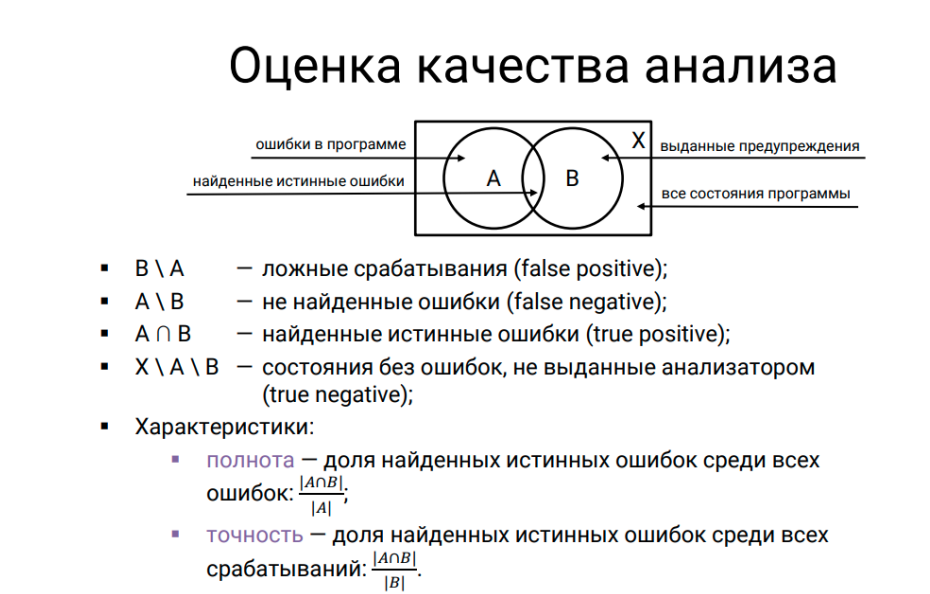
\includegraphics[width=\linewidth]{pics/quality_check.png}

Чувствительность к пути — способность анализа различать разные пути в программе.

Чувствительность к потоку — способность анализа различать порядок следования операторов.

Чувствительность к контексту — способность анализа различать разные вызовы одной функции.

\begin{itemize}
    \item Цель обнаружения ошибки — её устранение.
    \item Ошибка обнаруживается в месте её проявления в программе (выполнение некорректного действия).
    \item Исправление может требоваться в другом месте.
    \item Путь распространения ошибки — поток данных в программе, приведший к ошибке, делится на 3 части:
    \begin{itemize}
        \item[*] источник (source) — место инициализации переменных, значения которых привели к ошибке;
        \item[*] распространение (propagation) — операторы, участвовавшие в обработке/передаче значений, которые привели к ошибке;
        \item[*] сток, место проявления ошибки (sink) — оператор, приводящий к ошибке.
    \end{itemize}
\end{itemize}